% Venue target: LM4Sci 2026 (COLM 2026 template). Preprint mode: shows authors, no line numbers.
\documentclass{article}
\usepackage[preprint]{colm2026_conference}

\usepackage{microtype}
\usepackage{booktabs}
\usepackage{graphicx}
\usepackage{flafter}
\usepackage{float}
\usepackage{hyperref}
\usepackage{url}
\usepackage{xcolor}
\usepackage{tikz}
\usetikzlibrary{arrows.meta,positioning}

\definecolor{darkblue}{rgb}{0, 0, 0.5}
\definecolor{figurefill}{RGB}{246,248,251}
\definecolor{figureline}{RGB}{50,63,83}
\definecolor{figureaccent}{RGB}{226,236,249}
\definecolor{figuregreen}{RGB}{232,246,239}
\definecolor{figureamber}{RGB}{252,240,223}
\hypersetup{colorlinks=true, citecolor=darkblue, linkcolor=darkblue, urlcolor=darkblue}
\newcommand{\pending}{\textcolor{gray}{--}}
\renewcommand{\paragraph}[1]{%
  \par\addvspace{0.42\baselineskip}%
  \noindent\textbf{#1}\par\nobreak\vspace{-0.28\baselineskip}%
}

\title{Ranked Differential Diagnosis Across Frontier LLMs:\\ A Contamination-Controlled Neurology and Psychiatry Benchmark, and a Source-Grounded Retrieval Harness}
\author{\parbox{\linewidth}{\centering Santosh Gupta\\[2pt] \normalfont\texttt{SanGupta.ML@gmail.com}}}
\date{}

\begin{document}

\maketitle

\begin{abstract}
We evaluate frontier large language models on open-ended clinical diagnosis from peer-reviewed
\emph{neurology and psychiatry} case reports, scoring the full \emph{ranked differential} (top-1 through
top-5) rather than a single label. We build the benchmark by using an LLM (DeepSeek V4 Pro) to turn
published case reports into diagnostic challenges, then filter for answer leakage and for cases whose
diagnosis is not derivable from the prompt when evaluated against the case study from which it was created;
every retained case is a report published after every evaluated model's training cutoff, so it cannot have
been seen in pretraining. On a 68-case hard set
(cases DeepSeek V4 Flash fails closed-book), we evaluate seven frontier models---it plus DeepSeek V4 Pro,
Gemini 3.5 Flash and 3.1 Pro, Claude Opus 4.8, and GPT-5.4 and 5.5---and report how they distribute correct
answers across ranks. The central finding is that models differ not only in accuracy but in \emph{where they
place the correct diagnosis}: some surface it as their most confident (top-1) prediction, while others uncover
it lower in a broader list, so the model ordering re-arranges as the rank cutoff grows.
We then present ClinicalHarness, a retrieval-guided pipeline that pairs an LLM with PubMed/PMC retrieval and
a cheap per-paper reader. A core feature is that it grounds each diagnosis in citable literature the clinician
can verify---a cheap reader screens retrieved papers per case and returns a mean of about ten relevant
sources (rejecting roughly 73\% as irrelevant)---and it improves top-5 ranked accuracy for all three
answerers we could run at pipeline scale, most where the base model is weakest.
\end{abstract}

\section{Introduction}

Medical LLMs perform well on board-style multiple-choice and short-vignette diagnosis
\citep{MedPaLM,MedMCQA,PubMedQA}. Open-ended diagnosis from a real case report is harder: there are no
options, the differential matters, and the answer is a specific named entity at a particular granularity.
These systems should support a clinician rather than diagnose autonomously, and useful support is both
\emph{thorough} and \emph{verifiable}: a short ranked list of plausible diagnoses helps more than a single
best guess, and a diagnosis backed by sources the clinician can check helps more than an unsupported
assertion. Most evaluations reward neither---they score a single label with no provenance. We therefore score the whole ranked differential (top-1 through top-5) and ask two
questions. First, as a benchmark: how do frontier models compare when we credit a correct diagnosis
appearing anywhere in their top-1 through top-5, on cases chosen to be hard and guaranteed post-cutoff?
Second, as a systems question: can a retrieval harness raise a strong model's ranked recall?

The benchmark result is that frontier models re-order depending on the rank cutoff. A model that wins at
top-1 may be overtaken at top-5 by a model that holds the correct entity lower in a broader differential.
This is a statement about how a model distributes probability over a differential, not just about its
competence, and it is invisible if one scores only a single label.

\paragraph{Contributions.}
(1) A contamination-controlled, determinacy-audited benchmark of open-access neurology and psychiatry case
reports, scored on the full ranked differential. (2) A cross-model evaluation of seven frontier models at
top-1 through top-5 on a hard subset, with an interpretation of how their rank distributions differ,
tempered by the fact that their training is undisclosed. (3) ClinicalHarness, a retrieval-guided pipeline that
grounds each diagnosis in citable PubMed/PMC sources and improves top-5 ranked accuracy for every answerer we
ran. Benchmark and code are released (\S\ref{sec:data}).

\paragraph{Related work.}
This work connects medical LLM evaluation \citep{MedPaLM,MedMCQA,PubMedQA}, retrieval-augmented generation
\citep{RAG}, self-consistency and multi-agent deliberation \citep{SelfConsistency,MultiAgentDebate}, and
LLM-as-judge evaluation \citep{GEval,JudgeBias}. Our angle is ranked-differential scoring of open-ended
neurology/psychiatry diagnosis under contamination control.

\section{Benchmark Construction}\label{sec:bench}

The benchmark turns published case reports into redacted diagnostic challenges, then audits each challenge
for solvability. Figure~\ref{fig:benchmark} summarizes the pipeline.

\begin{figure}[t]
  \centering
  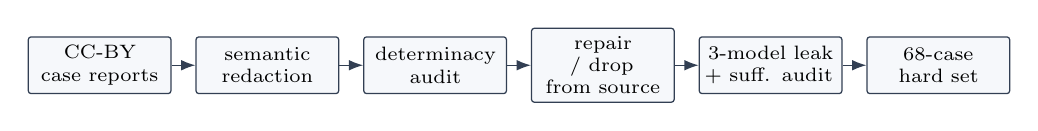
\begin{tikzpicture}[
    font=\scriptsize,
    node distance=0.025\linewidth,
    box/.style={draw=figureline, fill=figurefill, rounded corners=1pt, line width=0.45pt,
      align=center, inner sep=3pt, text width=0.132\linewidth, minimum height=0.72cm},
    arrow/.style={-{Latex[length=1.8mm]}, draw=figureline, line width=0.5pt}
  ]
    \node[box] (source) {CC-BY\\case reports};
    \node[box, right=of source] (redact) {semantic\\redaction};
    \node[box, right=of redact] (det) {determinacy\\audit};
    \node[box, right=of det] (repair) {repair / drop\\from source};
    \node[box, right=of repair] (audit) {3-model leak\\+ suff. audit};
    \node[box, right=of audit] (hard) {68-case\\hard set};
    \draw[arrow] (source) -- (redact);
    \draw[arrow] (redact) -- (det);
    \draw[arrow] (det) -- (repair);
    \draw[arrow] (repair) -- (audit);
    \draw[arrow] (audit) -- (hard);
  \end{tikzpicture}
  \caption{Benchmark construction. CC-BY case reports are turned into challenges by an LLM, audited for
  determinacy (is the answer derivable from the prompt?), repaired from the source or dropped, and---for the
  cross-model set---adversarially audited by three frontier models for answer leakage and insufficiency
  before a hand-checked drop/mend pass.}
  \label{fig:benchmark}
\end{figure}

\paragraph{Sourcing and licensing.} Cases derive from strictly CC-BY open-access neurology and psychiatry
case reports indexed in PubMed Central; each source paper yields one challenge. Each case stores a structured
gold diagnosis with aliases (for matching) and retains its source provenance (PMCID, DOI) so every challenge
can be traced and re-audited.

\paragraph{Challenge creation.} We use an LLM (DeepSeek V4 Pro) to rewrite each source case report into a
diagnostic challenge that withholds the diagnosis while keeping the clinical evidence needed to reach it.
The model reads the full report and reproduces the presentation, workup, and findings up to the point of
diagnosis, removing only the answer and any statement that gives it away.

\paragraph{Determinacy: is the answer in the prompt?} The key validity question is whether a challenge is
\emph{determinate}---whether every clinical fact required to reach the gold (a ``discriminator'') is present
in the prompt. This can only be judged by reading the \emph{entire} source case report against the
challenge, since a discriminator that lives only in the source and is missing from the challenge makes the
case unanswerable for any system, and so a benchmark defect rather than a model failure. The most common
defect is asking for an entity whose defining test result is withheld. For example, a prompt might present a
full phenotype, state that a gene panel ``was sent,'' and ask for the specific gene---but never give the
sequencing result, where the gene is not inferable from a phenotype shared with near neighbours (such as
DJ-1/PARK7 versus PRKN versus PINK1 in autosomal-recessive early-onset Parkinson's). A genuine reasoning
failure is the opposite: all discriminators are present and the model still picks the wrong entity. Only the
second should count against a model.

\paragraph{Repair or drop.} DeepSeek V4 was used to validate determinacy: it reads the challenge, the gold,
and the source full text and flags non-determinate cases. Each flagged case is then either repaired from the source---adding the
missing deciding result (the sequencing result, antibody titre, or biopsy finding) so the gold becomes
reachable, or reframing the question to the determinable next step---or dropped when no source-grounded
repair is possible. Repairs never relax the gold on the evaluation set. Re-auditing one 349-case batch
flagged about a quarter of cases; 34 were repaired from source and 16 were dropped.

\paragraph{Adversarial audit of the cross-model set.} For the cross-model comparison we begin with cases
that DeepSeek V4 Flash fails closed-book, then audit them with three frontier models---GPT-5.4, GPT-5.5, and
Claude Opus 4.8---each scoring two independent defects: \emph{leakage} (the prompt gives the answer away) and
\emph{insufficiency} (the prompt cannot determine the gold). Because automated auditors over-flag, every
flag is reviewed by hand against the source under a fixed rule: drop a case only when the prompt directly
reveals the target or the gold is not derivable; repair a case only when a source-grounded edit removes the
leak or supplies the missing fact without changing the gold; otherwise keep it. Typical drops are cases
where histology and molecular testing in the prompt already name the diagnosis; typical repairs delete a
post-question sentence that reveals the outcome, or move a required result to before the question. The
result is 13 drops and 11 source-grounded repairs, leaving the 68-case set used throughout.

\paragraph{Selection funnel and an economic-filter assumption.} The 68 cases are the survivors of a
deliberate cost-saving filter (Figure~\ref{fig:benchmark}). Across two post-cutoff batches we began with
\textbf{399} case challenges and kept only the \textbf{81} that DeepSeek V4 Flash---a cheap, lower-capacity
model---failed closed-book---discarding the 318 cases Flash solved---and the adversarial audit then reduced these to \textbf{68}. The rationale is
economic: running every frontier model on all 399 cases is costly, and the working assumption is that cases
a cheap model already solves are unlikely to discriminate among stronger models, so concentrating the
expensive frontier evaluation on the cheap model's failures saves budget while retaining the hard cases.
This assumption is not guaranteed---a frontier model may fail a case Flash solves, or vice versa, so the
filter could both miss discriminating cases and over-represent Flash-specific weaknesses. We flag it as a
deliberate but unverified design choice; a fuller study would evaluate all models on the entire pool.

\paragraph{Why a ranked differential.} For the near-neighbour cases above, the correct entity is often
already among a model's candidates even when its single best guess is wrong. Crediting a diagnosis that
appears anywhere in a ranked top-5 measures whether the system surfaced the right answer at all, and avoids
penalising it for the granularity of the single \#1 choice. We score top-1 through top-5 throughout.

\paragraph{Composition.} Table~\ref{tab:compose} characterizes the set, and Figure~\ref{fig:topics} shows
its etiologic-class frequencies. It is intentionally broad: cases span a broad range of conditions (Figure~\ref{fig:topics} shows the etiologic-class
breakdown), and across the 64 source papers carrying author keywords there are 338 distinct keywords with
almost no repetition. Patients
span pediatric to geriatric (age median 48, range 4--95) and both sexes. Recent reports are not yet
MeSH-indexed, so we report author keywords and derived classes in place of MeSH headings.

\begin{figure}[t]
  \centering
  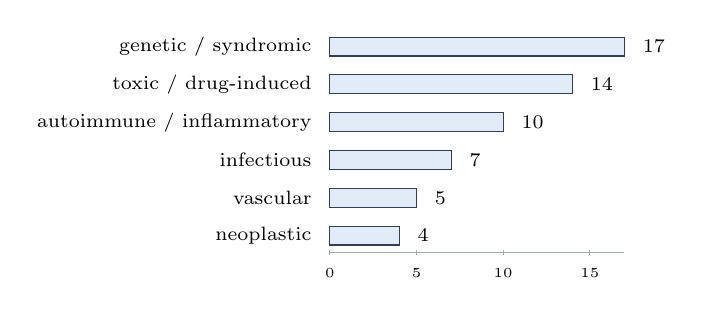
\begin{tikzpicture}[font=\scriptsize, x=0.22cm, y=0.48cm]
    \draw[figureline!45, line width=0.35pt] (0.5,0.35) -- (17.5,0.35);
    \foreach \x in {0,5,10,15} {
      \draw[figureline!45, line width=0.35pt] ({0.5+\x},0.28) -- ({0.5+\x},0.42);
      \node[anchor=north, font=\tiny] at ({0.5+\x},0.18) {\x};
    }
    \node[anchor=east, align=right] at (0,5.8) {genetic / syndromic};
    \draw[draw=figureline, fill=figureaccent, line width=0.4pt] (0.5,5.55) rectangle (17.5,6.05);
    \node[anchor=west] at (18.0,5.8) {17};
    \node[anchor=east, align=right] at (0,4.8) {toxic / drug-induced};
    \draw[draw=figureline, fill=figureaccent, line width=0.4pt] (0.5,4.55) rectangle (14.5,5.05);
    \node[anchor=west] at (15.0,4.8) {14};
    \node[anchor=east, align=right] at (0,3.8) {autoimmune / inflammatory};
    \draw[draw=figureline, fill=figureaccent, line width=0.4pt] (0.5,3.55) rectangle (10.5,4.05);
    \node[anchor=west] at (11.0,3.8) {10};
    \node[anchor=east, align=right] at (0,2.8) {infectious};
    \draw[draw=figureline, fill=figureaccent, line width=0.4pt] (0.5,2.55) rectangle (7.5,3.05);
    \node[anchor=west] at (8.0,2.8) {7};
    \node[anchor=east, align=right] at (0,1.8) {vascular};
    \draw[draw=figureline, fill=figureaccent, line width=0.4pt] (0.5,1.55) rectangle (5.5,2.05);
    \node[anchor=west] at (6.0,1.8) {5};
    \node[anchor=east, align=right] at (0,0.8) {neoplastic};
    \draw[draw=figureline, fill=figureaccent, line width=0.4pt] (0.5,0.55) rectangle (4.5,1.05);
    \node[anchor=west] at (5.0,0.8) {4};
  \end{tikzpicture}
  \caption{Etiologic-class frequency across the 68 cases (non-exclusive). Recent reports are not yet
  MeSH-indexed, so we use derived class labels and author keywords rather than
  MeSH headings.}
  \label{fig:topics}
\end{figure}

\begin{table}[t]
\centering
\resizebox{\columnwidth}{!}{%
\begin{tabular}{ll}
\toprule
Dimension & Distribution (of 68 cases) \\
\midrule
Post-cutoff batches & two batches (33, 35); all published after every model's cutoff \\
License & CC-BY (68/68) \\
Patient sex & 36 female, 28 male \\
Patient age & median 48, range 4--95 (pediatric to geriatric) \\
Author keywords & 338 unique across 64 papers; long-tail (no concept recurs $>$2$\times$ except ``case report'') \\
Source venues & Cureus 24, Frontiers family 11, Elsevier 4, Hindawi 3, others \\
\bottomrule
\end{tabular}}
\caption{Composition of the 68-case cross-model set: a long tail of specific conditions rather than a few
concentrated topics.}
\label{tab:compose}
\end{table}



\section{Cross-Model Benchmark Results}\label{sec:cross}

We score each model's bare (no retrieval) ranked differential at temperature 0 on all 68 cases, crediting a
diagnosis that appears at rank $\le n$. Scoring uses an alias-aware LLM judge with lexical fallback, using
majority-of-3 judging because single-vote judging at temperature 0 is itself mildly stochastic.

\subsection{Interpretation: models re-order as the rank cutoff grows}

\begin{table}[H]
\centering
\begin{tabular}{lrrrrr}
\toprule
Model & top-1 & top-2 & top-3 & top-4 & top-5 \\
\midrule
GPT-5.4            & 47 & 53 & 55 & 56 & \textbf{57} \\
Gemini 3.5 Flash   & 29 & 42 & 49 & 52 & \textbf{54} \\
GPT-5.5            & 43 & 46 & 49 & 51 & 51 \\
Claude Opus 4.8    & 33 & 41 & 46 & 48 & 50 \\
DeepSeek V4 Pro    & 31 & 40 & 43 & 44 & 47 \\
Gemini 3.1 Pro     & 29 & 38 & 41 & 41 & 44 \\
DeepSeek V4 Flash  & 17 & 27 & 32 & 36 & 40 \\
\bottomrule
\end{tabular}
\caption{Bare ranked-differential accuracy (count of 68) at each rank cutoff, temperature 0, majority-of-3
judge. The set is failure-selected (DeepSeek V4 Flash top-1 failures), so absolute numbers index difficulty,
not general quality.}
\label{tab:bare}
\end{table}

Table~\ref{tab:bare} is more revealing read \emph{across} columns than down any one. We offer the following
as interpretation, not mechanism.

\paragraph{Models differ in how peaked their differential is.} GPT-5.5 is nearly flat after top-3
($49\to51\to51$): when it is right, it is right early, and extra ranks add little. Gemini 3.5 Flash is the
opposite---it starts low at top-1 (29) but gains steadily to 54 at top-5, frequently having the correct
entity but placing it lower in the list. The two cross over: GPT-5.5 leads Flash at top-1 (43 vs.\ 29) but
trails it at top-5 (51 vs.\ 54).

\paragraph{The top-1 to top-2 jump separates the spread models.} The per-rank gains expose the mechanism.
Gemini 3.5 Flash gains $+13$ from top-1 to top-2---the largest single-rank jump of any model---and $+25$
overall, climbing from sixth at top-1 (below DeepSeek Pro's 31) to second by top-3 and holding second at
top-5, overtaking DeepSeek Pro, Opus, and GPT-5.5. A $+13$ jump means 13 of 68 cases where the model's rank-1
was wrong but its rank-2 was right: near misses in which the correct diagnosis was the model's close second,
a ranking choice rather than ignorance. The two cheap ``Flash'' models climb most (Gemini Flash $+25$,
DeepSeek Flash $+23$); the large GPT-5.x models climb least (GPT-5.4 $+10$, GPT-5.5 $+8$, the latter flat
after top-3), behaving like committed single-answer models. A single-label leaderboard would place Gemini
Flash fifth or sixth; on the differential it is second.

\paragraph{Further observations, offered without mechanism.} Two patterns stand out. Within a family the
cheaper model can win: Gemini 3.5 \emph{Flash} reaches top-5 54, ten points above Gemini 3.1 \emph{Pro} (44),
so capability tier and price do not predict differential quality here. And even the selection model recovers
with ranks: DeepSeek V4 Flash defines the set---it fails these at top-1 by construction---yet recovers 40/68
at top-5, so for much of its ``failures'' the knowledge was in the differential and the failure was one of
selection. We were genuinely surprised that the smallest, cheapest model (Gemini Flash) climbed from sixth at
top-1 to second at top-5, and that the earlier GPT-5.4 edged the later GPT-5.5; but the training data and
architectures of these models are undisclosed, so we can establish that their rank distributions differ
without being able to say why. This is also a failure-selected, single-seed set, so fine rank distinctions
should not be over-read.



\section{ClinicalHarness}\label{sec:harness}

ClinicalHarness is a retrieval-guided diagnostic pipeline (Figure~\ref{fig:harness}) that uses two distinct
roles: a \emph{primary LLM} that reasons about the case and produces the differential, and a cheap, separate
\emph{reader LLM} (DeepSeek V4 Flash in our runs) that screens individual retrieved papers. The split exists
because most retrieved papers are irrelevant: the reader judges each paper against the current case and
passes back only the small distillate it deems useful, so the primary LLM is never flooded with raw paper
text and can read many papers per case on a small context.

\begin{figure}[t]
  \centering
  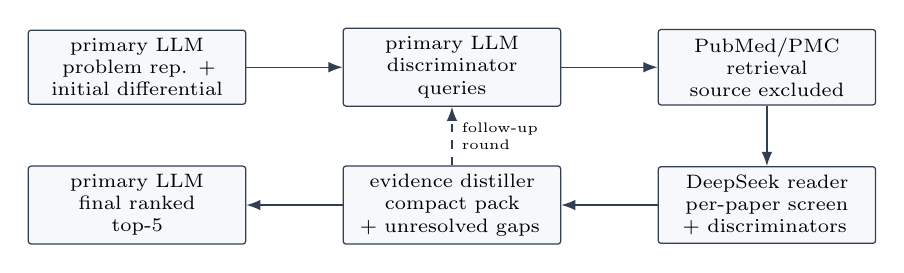
\begin{tikzpicture}[
    font=\scriptsize,
    box/.style={draw=figureline, fill=figurefill, rounded corners=1pt, line width=0.45pt,
      align=center, inner sep=3pt, text width=2.55cm, minimum height=0.82cm},
    arrow/.style={-{Latex[length=1.8mm]}, draw=figureline, line width=0.5pt}
  ]
    \node[box] (initial) at (0,1.75) {primary LLM\\problem rep. +\\initial differential};
    \node[box] (query) at (4.0,1.75) {primary LLM\\discriminator\\queries};
    \node[box] (retrieve) at (8.0,1.75) {PubMed/PMC\\retrieval\\source excluded};
    \node[box] (reader) at (8.0,0) {DeepSeek reader\\per-paper screen\\+ discriminators};
    \node[box] (distill) at (4.0,0) {evidence distiller\\compact pack\\+ unresolved gaps};
    \node[box] (answer) at (0,0) {primary LLM\\final ranked\\top-5};
    \draw[arrow] (initial) -- (query);
    \draw[arrow] (query) -- (retrieve);
    \draw[arrow] (retrieve) -- (reader);
    \draw[arrow] (reader) -- (distill);
    \draw[arrow] (distill) -- (answer);
    \draw[arrow, dashed] (distill.north) -- node[right, font=\tiny, align=left] {follow-up\\round} (query.south);
  \end{tikzpicture}
  \caption{ClinicalHarness pipeline. The primary LLM forms an initial differential and targeted queries;
  retrieval runs in eval mode (the source paper is excluded); a cheap reader LLM screens each retrieved paper
  and returns only case-relevant findings; a distiller compiles the evidence and decides whether to run
  another retrieval round; the primary LLM then produces the final ranked differential.}
  \label{fig:harness}
\end{figure}

\paragraph{1. Problem representation and initial differential (primary LLM).} The primary LLM reads the case
and produces a structured problem representation and an initial, pre-retrieval differential of candidate
diagnoses. A feature-indexed preset selector first maps the case to a diagnostic family (for example acute
neurological emergency, infection/inflammation, or rare tumour), which conditions the prompt toward the
relevant discriminators.

\paragraph{2. Query generation (primary LLM).} From the problem representation the primary LLM proposes
targeted PubMed/PMC queries. These favour \emph{discriminator} queries that separate the leading hypothesis
from its closest mimics, rather than queries that merely confirm the leading hypothesis.

\paragraph{3. Retrieval in eval mode.} Queries run against PubMed/PMC. Eval mode enforces contamination
control: the case's own source paper is excluded by PMCID, DOI, title, and generic-mimic filters, so the
system cannot retrieve the answer. The harness may search for syndromes, discriminators, imaging patterns,
or treatment guidelines, but never for the source itself.

\paragraph{4. Per-paper screening (reader LLM).} Each retrieved paper is screened in its own isolated
reader call. The reader returns a compact structured note only when the paper is judged relevant to
\emph{this} case---a short relevant excerpt, the discriminators it supplies, which hypotheses it supports or
refutes, any candidate diagnosis it raises that is not yet in the differential, and follow-up queries it
suggests. The vast majority of retrieved papers contain no usable information for the case; those are
discarded, and only the relevant distillates pass back. The full paper text never re-enters the primary
LLM's context.

\paragraph{5. Evidence distillation and adaptive rounds.} The relevant per-paper notes are compiled into a
single evidence pack that summarises the decisive discriminators and the still-unresolved mimic pairs, and
decides whether another retrieval round is warranted. When a discriminator remains unresolved, the system
issues a follow-up query plan and runs another round (up to a bounded maximum); otherwise it finalises.

\paragraph{6. Final ranked differential (primary LLM).} The primary LLM receives the evidence pack together
with its earlier problem representation and emits a ranked top-5 differential and a rank-1 final diagnosis.
Retrieval may add literature-surfaced candidates and re-order the list relative to the pre-retrieval
differential.

\paragraph{Development.} The harness components were developed and tuned on earlier validated case batches
that predate this benchmark---roughly 350 development cases---using DeepSeek V4 Pro as a strong primary LLM
to surface and fix failure modes. Tuning was frozen before the post-cutoff 68-case set was constructed, so
no component was optimised on the evaluation cases.

\section{Harness Results: Bare versus Harness (top-5)}\label{sec:harnessresults}

We compare each model's bare top-5 (Table~\ref{tab:bare}) against its top-5 \emph{inside} the harness as the
primary LLM, paired with the cheap DeepSeek reader and the same majority-of-3 judge, on the same 68 cases.
Both sides are temperature 0.

\begin{table}[t]
\centering
\begin{tabular}{llrrrrr}
\toprule
Model (primary LLM) & & top-1 & top-2 & top-3 & top-4 & top-5 \\
\midrule
Gemini 3.5 Flash  & bare  & 28 & 44 & 51 & 54 & 56 \\
                  & fused & 28 & 44 & 51 & 54 & \textbf{57} \\
\midrule
DeepSeek V4 Pro   & bare  & 31 & 39 & 45 & 45 & 48 \\
                  & fused & 31 & 39 & 45 & 45 & \textbf{50} \\
\midrule
DeepSeek V4 Flash & bare  & 17 & 27 & 34 & 39 & 43 \\
                  & fused & 17 & 27 & 34 & 39 & \textbf{46} \\
\bottomrule
\end{tabular}
\caption{Bare versus do-no-harm \emph{fused} ranked accuracy (count of 68) at each cutoff, temperature 0,
same majority-of-3 judge within each run. The fusion preserves the model's bare top-4 and fills only the
fifth slot with the harness's single highest-confidence retrieval-surfaced diagnosis absent from the bare
list, so top-1 through top-4 are identical to bare and only top-5 moves. Scores are within-run (the bare
differential re-judged by the same judge), so they differ by $\le 3$ from the standalone bare scores in
Table~\ref{tab:bare}. The harness ran end-to-end only for the answerers shown; the others were evaluated
bare only.}
\label{tab:harness}
\end{table}

\paragraph{Why not all models in the harness.} The harness is a multi-call pipeline---an initial
differential, query generation, per-paper reader screens across several retrieval rounds, a distiller, and a
final reranker---so it issues roughly an order of magnitude more model calls (and tokens) per case than a
single bare query. At that volume, running Claude Opus, the GPT-5.x models, or Gemini 3.1 Pro as the primary
LLM was cost-prohibitive; all remain affordable in the single-call bare setting. We therefore report all
seven models bare (Table~\ref{tab:bare}) and restrict the harness comparison to the Gemini Flash and DeepSeek
answerers.

\paragraph{Do-no-harm fusion.} We combine the harness with the model's own differential conservatively: we
keep the model's bare top-4 unchanged and let the harness fill only the fifth slot, with the single
highest-confidence diagnosis the retrieval surfaced that the model did not already list. By construction this
cannot demote a confident bare candidate---top-1 through top-4 are identical to bare---so the harness
contributes exactly where it should, recovering a missed diagnosis into the last slot. This improves top-5
for all three answerers (Table~\ref{tab:harness}), and the gain grows as the base model weakens---$+1$ for
the strongest answerer (Gemini Flash), $+2$ for DeepSeek V4 Pro, and $+3$ for the weakest (DeepSeek V4
Flash)---consistent with retrieval helping most where the base model has a genuine knowledge gap.
(Substituting the harness's reordered differential wholesale instead of fusing it \emph{lowers} ranked
accuracy, by crowding the model's own correct diagnoses down the list; \S\ref{sec:disc}.)

\paragraph{Source-grounded diagnosis.} Beyond accuracy, a central feature of the harness is that every
diagnosis arrives with the literature it rests on, so a clinician can check the reasoning rather than trust
an opaque guess. The reader screens each retrieved paper against the case and returns only the relevant
ones with the specific discriminators they supply: a mean of about 10 grounding sources per case (standard
deviation $\sim$9.5, range 0--39), selected from a mean of $\sim$39 retrieved papers of which the reader
rejects roughly 73\% as irrelevant. These retained papers, attached to the final differential by PMCID/DOI,
are the provenance a clinician can follow to verify each candidate.

\section{Discussion}\label{sec:disc}

Two themes recur. First, differential structure is a model property: frontier models that look similar on a
single label differ markedly in how they spread correct answers across a ranked list, and the appropriate
metric depends on whether the consumer wants one label or a short differential. Concretely, the choice of
metric re-orders the leaderboard---at top-1 the GPT-5.x models lead (GPT-5.4 first with 47, GPT-5.5 second
with 43) while Gemini 3.5 Flash sits near the bottom (29); by top-5 Gemini Flash has climbed to second (54)
and GPT-5.5 has fallen behind it (51)---so a single-label evaluation mis-ranks exactly the models that are
most useful when the deliverable is a differential for a clinician to weigh.

Second, augmentation must be integrated conservatively. Replacing a strong model's differential with
retrieval output can crowd its own correct diagnoses down the list, because a model with rich internal
medical knowledge already holds a broader differential than a few distilled passages convey. A do-no-harm
fusion that preserves the model's confident candidates and lets retrieval add only a diagnosis the model
missed avoids this and yields a consistent top-5 gain (Table~\ref{tab:harness}), largest where the base model
is weakest---supporting the reading that external evidence complements parametric knowledge at the margin
rather than replacing it. How far that margin extends---how much a stronger reader, broader retrieval, or a
multi-slot fusion can add without reintroducing interference---is open work.

\section{Limitations}

The hard set is failure-selected, so absolute scores index difficulty rather than general quality, and small
rank gaps are within judge noise. Mechanistic claims about why model differentials differ are out of
reach because training details are undisclosed. Published case reports are retrospective and selected for
novelty, so this is a test of diagnostic reasoning from curated evidence, not a clinical decision-support
trial. The harness fusion is deliberately conservative (it touches only the fifth slot); a multi-slot fusion
could add more but risks reintroducing the interference that single-list substitution showed.

\section{Data, Code, and Ethics}\label{sec:data}

The benchmark and ClinicalHarness code are released at
\url{https://github.com/Santosh-Gupta/ClinicalOrchestra}. Runs persist prompts, model
responses, retrieval provenance, and scoring records so every reported number is traceable to an artifact.
This work evaluates retrospective, published case reports; it is not a clinical decision-support system and
must not be used for patient care without prospective validation and governance.

\bibliographystyle{colm2026_conference}
\bibliography{../paper_references}

\appendix

\section{Benchmark construction pipeline components (Figure~\ref{fig:benchmark})}\label{app:bench-components}
The six stages of Figure~\ref{fig:benchmark}, end to end:
\begin{description}
\item[CC-BY case reports.] The raw input: strictly CC-BY open-access neurology and psychiatry case reports
indexed in PubMed Central, each retained with its full text, PMCID, and DOI. One source paper becomes one
challenge.
\item[Semantic redaction.] An LLM (DeepSeek V4 Pro) rewrites each report into a diagnostic challenge that
reproduces the presentation, workup, and findings up to the point of diagnosis while removing the stated
diagnosis and any sentence that gives it away (final ``the diagnosis was X'' lines, disease-naming treatment,
and similar tells).
\item[Determinacy audit.] A check, made against the \emph{full} source, that every clinical fact required to
reach the gold (every ``discriminator'') survives in the redacted challenge---so the case is solvable from
the prompt alone and a wrong answer reflects reasoning rather than a fact missing from the prompt.
\item[Repair / drop from source.] Non-determinate challenges are either repaired from the source---re-inserting
the missing deciding result (a sequencing result, antibody titre, or biopsy finding) or reframing to the
determinable next step---or dropped when no source-grounded repair is possible. Repairs never relax the gold.
\item[3-model leak + sufficiency audit.] For the cross-model set, three frontier models (GPT-5.4, GPT-5.5,
Claude Opus 4.8) independently flag two defects per case---leakage (the prompt reveals the answer) and
insufficiency (the prompt cannot determine the gold)---and every flag is reviewed by hand against the source
before any drop or repair.
\item[68-case hard set.] The surviving challenges, restricted to cases the cheap DeepSeek V4 Flash fails
closed-book, form the 68-case evaluation set used throughout. The harness pipeline (Figure~\ref{fig:harness})
is described stage-by-stage in \S\ref{sec:harness}.
\end{description}


\end{document}
